\documentclass{article}

\usepackage[utf8]{inputenc}
\usepackage{amsfonts}
\usepackage{graphicx}
\usepackage{amsthm}
\usepackage{amsmath}
\usepackage{wrapfig}
\usepackage{cleveref}
\usepackage{subcaption}
\usepackage{listings}
\usepackage{xspace}
\usepackage{pifont}      % Provides the ding symbol used for comments
\usepackage{xcolor}       % Used to highlight comments
\usepackage{algorithm}
\usepackage[noend]{algpseudocode}
\usepackage{algorithmicx}
\usepackage{prftree}
\usepackage{stmaryrd}

\newtheorem{theorem}{Theorem}
\theoremstyle{definition}
\newtheorem{proposition}{Proposition}
\newtheorem{definition}{Definition}
\newtheorem{example}{Example}
\newtheorem{note}{Note}

\newcommand{\ite}[3]{\texttt{if}\ #1\ \texttt{then}\ #2\ \texttt{else}\ #3\ \texttt{end}}
% \newcommand{\ite}[3]{#1 \to #2 + #3}
\newcommand{\para}[2]{#1 \ ||\ #2}
\newcommand{\config}[0]{K}
\newcommand{\state}[0]{S}
\newcommand{\ownin}[0]{I}
\newcommand{\ownout}[0]{O}
\newcommand{\prefix}[1]{\textsf{Prefix}(#1)}
\newcommand{\waitgraph}[0]{\textsf{Wait}}

\newcommand{\bool}[0]{\textsf{Bool}}
\newcommand{\true}[0]{\textsf{true}}
\newcommand{\false}[0]{\textsf{false}}
\newcommand{\arity}[1]{\textsf{arity}(#1)}
\newcommand{\terms}[1]{\textsf{Term}_{#1}}
\newcommand{\procs}[0]{\textsf{Proc}}
\newcommand{\sorts}[0]{\textsf{Sort}}
\newcommand{\symbols}[0]{\textsf{Symbol}}
\newcommand{\chans}[0]{\textsf{Chan}}

\newcommand{\interp}[2]{\llbracket #1 \rrbracket_{#2}}
\newcommand{\trans}[1]{\xrightarrow{\ #1\ }}

\newcommand{\partialtran}[3]{\overset{#1}{\rightsquigarrow}_{#2, #3}}

\def\sepr{|}
\DeclareMathOperator\eval{eval}
\def\epsi{\varepsilon}
\def\subst{\mathbin{\mapsto}}
\DeclareMathOperator\fv{fv}
\DeclareMathOperator\fc{fc}

%% Processes

\colorlet{cProc}{black}
\def\fProc#1{{\mathit{\color{cProc}#1}}}

\def\pIn#1(#2){#1(#2)}
\def\pOut#1[#2]{#1[#2]}
\def\pKw#1{\mathinner{#1}}
\def\pIf{\pKw{if}}
\def\pThen{\pKw{then}}
\def\pElse{\pKw{else}}
\def\pCall#1(#2){#1(#2)}
\def\pSubst#1{{\big[#1\big]}}

%% (Dataflow) Systems

\colorlet{cSys}{violet} % TODO: replace by color-blindness-friendly color.
\def\fSys#1{{\mathsf{\color{cSys}#1}}}

\title{Dataflow Deadlock}
\author{Zhengyao}
\date{July 2024}

\begin{document}

\maketitle

\section{Deadlocks}

For our purpose, we only care about a fixed set of processes with a fixed topology.
We fix a set of channel names $C$.
The syntax of processes is as follows:
\begin{align*}
    P ::=&\ 0 \\
        |&\ c?x. P & \text{Input} \\
        |&\ c!t. P & \text{Output} \\
        |&\ \ite{t}{P_1}{P_2} & \text{Branching} \\
        |&\ \alpha & \text{Process variable} \\
        |&\ \mu \alpha. P & \text{Recursion}
\end{align*}
The term $t$ is over a usual signature of integers and Booleans, for example.
We put a usual structural congruence over the syntax, including unfolding of recursion.
We define free variables and substitution the usual way ($c?x. P$ binds $x$ in $P$, and $\mu \alpha. P$ binds $\alpha$ in $P$).

We define how each closed process interacts with the environment using the following LTS, where $c?t$ is an input action, $c?t$ is an output action, and $\tau$ is a silent action.
\begin{gather*}
    c?x. P \trans{c?t} P[t/x] \qquad \text{for any term $t$} \\
    c!t. P \trans{c!t} P \\
    \ite{t}{P_1}{P_2} \trans{\tau} P_1 \qquad \text{if $t$ is true} \\
    \ite{t}{P_1}{P_2} \trans{\tau} P_2 \qquad \text{if $t$ is false} \\
\end{gather*}

A dataflow program is essentially a parallel composition of a fixed number of processes.
\begin{definition}[Dataflow Configuration]
    Suppose we have a set of processes $\{ P_i \}^n_{i = 1}$, a \emph{configuration} is a tuple $K = (\{ P_i \}^n_{i = 1}, \{ I_i \}^n_{i = 1}, \{ O_i \}^n_{i = 1})$, where
    \begin{itemize}
        \item $I_i, O_i \subseteq C$ are sets of channels.
        \item $I_1, \dots, I_n$ are disjoint; $O_1, \dots, O_n$ are disjoint.
        \item Each $P_i$ can only contain input prefix of $c?$ for $c \in I_i$, and output prefix $c!$ for $c \in O_i$.
        \item $I_1 \sqcup \dots \sqcup I_n = O_1 \sqcup \dots \sqcup O_n$.
    \end{itemize}
\end{definition}
We use $K[i \mapsto P]$ to denote a configuration $K$ with the $i$-th process replaced by $P$.

We define a reduction on configurations (basically like a parallel composition of the $n$ processes):
\begin{gather*}
    \begin{prftree}
        {P_i \trans{c?t} P'_i}
        {\qquad P_j \trans{c!t} P'_j}
        {\qquad i \ne j}
        {K[i \mapsto P_i, j \mapsto P_j] \trans{} K[i \mapsto P'_i, j \mapsto P'_j]}
    \end{prftree} \\ \\
    \begin{prftree}
        {P_i \trans{\tau} P'_i}
        {K[i \mapsto P_i] \trans{} K[i \mapsto P'_i]}
    \end{prftree}
\end{gather*}

We say that a configuration has a deadlock if there is a cycle in the ``wait graph'' defined below.
\begin{definition}[Wait Graph]
    Given configuration $K = (\{ P_i \}^n_{i = 1}, \{ I_i \}^n_{i = 1}, \{ O_i \}^n_{i = 1})$, the wait graph $\waitgraph(K) = (V, E, L)$ is a labelled directed graph with vertices $V = \{ 1, \dots, n \}$, and there is an edge $(i, j) \in E$ with label $L(i, j) = c$ iff
    \begin{itemize}
        \item $P_i \trans{c?t} P'_i$, and $c \in O_j$ ($P_i$ waits for $P_j$ to send something), or
        \item $P_i \trans{c!t} P'_i$, and $c \in I_j$ ($P_i$ waits for $P_j$ to receive something).
    \end{itemize}
\end{definition}

\begin{definition}[Deadlock]
    A configuration $K = (\{ P_i \}^n_{i = 1}, \{ I_i \}^n_{i = 1}, \{ O_i \}^n_{i = 1})$ is in a \emph{deadlock} if $\waitgraph(K)$ has a cycle, and if the cycle length is two, we require that the labels of the two edges are distinct.
\end{definition}

Given an initial configuration $K$, we essentially want to check if there is a reachable configuration with deadlock.

\section{Semantics of RipTide Operators}

The semantics of the operators in RipTide (\cite{riptide}, Fig.~3) can be modelled as processes defined above:
\begin{itemize}
    \item All the arithmetic operators (also including select) read from all inputs, send to all outputs, and then repeat. For example, the addition operator has the behavior $\mathsf{Add} = a?x. b?y. c!(x + y). d!(x + y). \mathsf{Add}$, if it has two inputs $a$ and $b$ at different ``input ports'', and two outputs $c$ and $d$ connected to the same ``output port''.
    \item There are some memory operators (load ans store). On channels, they behave similar to arithmetic operators, but, in addition, they may read/write a globally shared memory, which is currently not modelled in the processes above.
    \item Finally and most importantly, there are some control-flow operators that can change input/output behavior depending on values received. Some examples include:
    \begin{itemize}
        \item Steer (inputs $a$, $d$; output $b$) reads an input from $a$, and a ``decider'' value from $d$. If the decider is true, it forwards the value from $a$ to $b$; otherwise it discards the value received:
        \begin{align*}
            \mathsf{Steer} =&\ a?x. \\
                            &\ d?y. \\
                            &\ \ite{y}{\\
                            &\ \qquad b!x. \mathsf{Steer} \\
                            &\ }{ \\
                            &\ \qquad \mathsf{Steer} \\
                            &\ }
        \end{align*}
        
        % \[
        %     \mathsf{Steer} = a?x. d?y. \ite{y}{b!x. \mathsf{Steer}}{\mathsf{Steer}}
        % \]
        \item Merge (inputs $d, a, b$; output $c$) first reads from the decider channel $d$. If it's true, then it read from the first input $a$ and forwads the value to $c$; otherwise it reads from the other input $b$, and forwards the value to $c$ (same output).
        \begin{align*}
            \mathsf{Merge} =&\ d?x. \\
                            &\ \ite{x}{\\
                            &\ \qquad a?y. c!y. \mathsf{Merge} \\
                            &\ }{ \\
                            &\ \qquad b?y. c!y. \mathsf{Merge} \\
                            &\ }
        \end{align*}
        % \[
        %     \mathsf{Merge} = d?x. \ite{x}{a?y. c!y. \mathsf{Merge}}{b?y. c!y. \mathsf{Merge}}
        % \]

        \item Carry (inputs $d, a, b$; output $c$) is exactly like a merge, except that initially it would always forward the first input.
        \begin{align*}
            \mathsf{CarryInit} =&\ a?x. c!x. \mathsf{CarryLoop} \\
            \mathsf{CarryLoop} =&\ d?x. \\
                                &\ \ite{x}{\\
                                &\ \qquad b?y. c!y. \mathsf{CarryLoop} \\
                                &\ }{ \\
                                &\ \qquad \mathsf{CarryInit} \\
                                &\ }
        \end{align*}

        \item Invariant (inputs $d, a$; output $b$) reads a value from the input, and continue sending the same value if the decider is true.
        \begin{align*}
            \mathsf{InvInit} =&\ a?x. b!x. \mathsf{InvLoop}(x) \\
            \mathsf{InvLoop}(x) =&\ d?y. \\
                                &\ \ite{y}{\\
                                &\ \qquad b!x. \mathsf{InvLoop}(x) \\
                                &\ }{ \\
                                &\ \qquad \mathsf{InvInit} \\
                                &\ }
        \end{align*}
    \end{itemize}
\end{itemize}

\section{Calculus}
\label{sec:calculus}

\subsection{Dataflow Systems}
\label{sec:calculus:systems}

We use $\fProc{a},\fProc{b},\ldots$ to denote channels, $\fProc{v},\fProc{w},\ldots$ to denote variables, $\fProc{e},\fProc{f},\ldots$ to denote expressions, $\fProc{X},\fProc{Y},\ldots$ to denote process definitions.
We write $\fProc{\tilde{a}}$ and $\fProc{\tilde{v}}$ to denote (comma-separated) sequences of zero or more channels and variables, respectively; we use $\fProc{\epsi}$ to denote the empty sequence.
Processes $\fProc{P},\fProc{Q},\ldots$ are defined as follows.
\[
    \begin{array}{@{}r@{}c@{}lr@{}}
        \fProc{P},\fProc{Q},\ldots & {}::={} &
        \fProc{0} & \text{inaction}
        \\
        & \sepr &
        \fProc{\pIn a(v) ; P} & \text{input}
        \\
        & \sepr &
        \fProc{\pOut \tilde{a}[e] ; P} & \text{output}
        \\
        & \sepr &
        \fProc{\pIf e \pThen P \pElse Q} & \text{conditional}
        \\
        & \sepr &
        \fProc{\pCall X(\tilde{a};\tilde{v})} & \text{process call}
    \end{array}
\]
Expressions are left unspecified, but may use variables.
We write $\eval(\fProc{e})$ to denote the evaluation of $\fProc{e}$ to a value.
Given $\fProc{w}$ a value, we write $\fProc{P \pSubst{v \subst w}}$ to denote the substitution of every occurrence of $\fProc{v}$ in $\fProc{P}$.
Input $\fProc{\pIn a(v) ; P}$ binds the occurrences of $\fProc{v}$ in $\fProc{P}$.
We write $\fv(\fProc{P})$ and $\fc(\fProc{P})$ to denote the sets of free variables and free channels in $\fProc{P}$, respectively.

A (dataflow) system $\fSys{S}$ is a tuple $\fSys{(Defs,Bufs,Procs)}$ where
\begin{itemize}
    \item $\fSys{Defs}$ is a set of process definitions $\fProc{X(\tilde{a};\tilde{v}) = P}$,
    \item $\fSys{Bufs}$ is a set of buffers, and % TODO: define buffers.
    \item $\fSys{Procs}$ is a set of processes.
\end{itemize}

\subsection{Deadlock}
\label{sec:calculus:deadlock}

% TODO: define closed systems.
% TODO: define deadlock.

\section{Examples and Non-Examples of Deadlocks}

The following are some cases considered as deadlocks or non-deadlocks in RipTide.
Some of them are best represented as dataflow graphs, so I am showing the figures instead of writing down the processes.

\paragraph{Unbalanced steer (deadlock)}

In the following dataflow graph, we have a steer operator \texttt{T} (whose behavior is defined in the last section), a producer operator \texttt{A} (which repeatedly sends outputs to its output channels), and a consumer operator \texttt{B} (which repeatedly receives inputs from the its input channels).
\begin{center}
    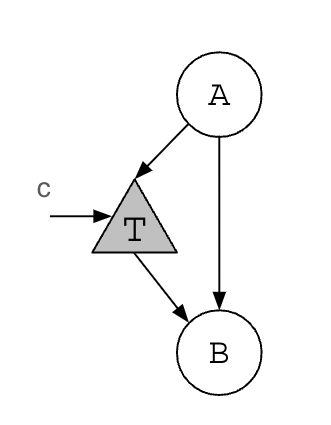
\includegraphics[width=0.3\textwidth]{steer-deadlock.png}
\end{center}

Due to the synchronous semantics, if the decider value \texttt{T} receives from $c$ is false, then we are in a dependency cycle: \texttt{A} waits for \texttt{B} to receive a value; \texttt{B} waits for \texttt{T} to send a value; and then \texttt{T} waits for \texttt{A} to send a value.

\paragraph{Branching (non-deadlock)}

The following dataflow graph is usually used for representing a branch in an imperative program.
The first operator \texttt{S} is a called a ``switch'' in dataflow literature.
It reads a value from $a$, and a decider from $b$, then it forwards the value from $a$ to $d$ if the decider is true; otherwise it forwards the value to $e$.
In RipTide the switch is split up to two steer gates, but here for simplicity we just use one operator.

In the rest of the graph, \texttt{A} and \texttt{B} can be considered as usualy arithmetic operators.
The operator \texttt{M} is a merge operator defined in the previous section: if $c$ is true, it forwards the value from $h$; otherwise it forwards the value from $f$.

\begin{center}
    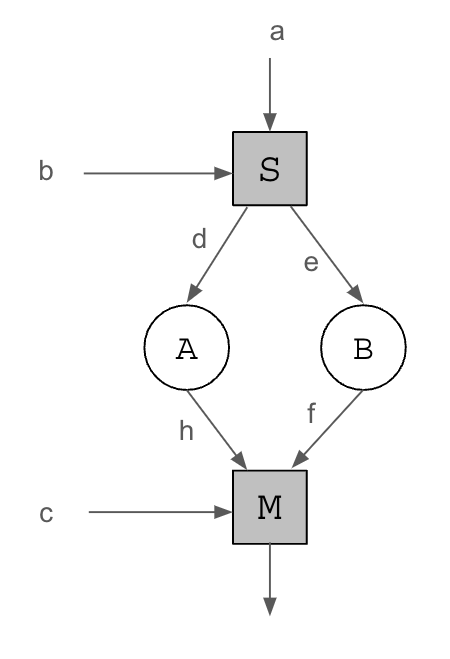
\includegraphics[width=0.4\textwidth]{branching.png}
\end{center}

In this case, usually $b$ and $c$ are connected to the same comparison operator (which might be computing a branching condition), and $b$ and $c$ should usually have the same Boolean value.
So if $b = c$, then every time either \texttt{A} or \texttt{B} will be executed, and there is no deadlock.

However, if the graph is connected incorrectly, and $b$ and $c$ may have different values, then we might be in a deadlock.
For example, if $b$ is true and $c$ is false, then \texttt{S} will try to send to \texttt{A}, but \texttt{M} will try to read from \texttt{B}, and we are stuck.

\paragraph{Loop (deadlock)}

This one is a canonical deadlock example used in literature.
We have two processes waiting for each other's input: $\para{\mu \alpha. a?x. b!x. \alpha}{\mu \beta. b?x. a!x. \beta}$.
This is also possible in a dataflow graph if two operators are connected incorrectly in a feedback loop without an initial value to ``kickstart'' the loop.

\paragraph{Loop (``good'' termination, but not deadlock)}

Cycles in a dataflow graph do not always cause deadlocks, and are actually required to represent loops in an imperative language.
Here is a perfectly correct dataflow graph compiled from an imperative program:
\begin{verbatim}
1.  i = 0
2.  while i < len
3.      B[i] = A[i] + 1
4.      i = i + 1
\end{verbatim}
where \texttt{B} and \texttt{A} are pointers or arrays in the global memory.

\begin{center}
    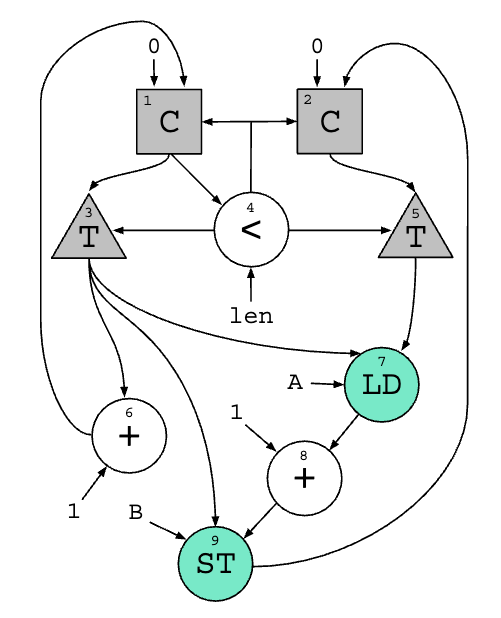
\includegraphics[width=0.4\textwidth]{loop.png}
\end{center}

In this graph, the carry operator indexed 1 represents the loop variable \texttt{i}: initially it has a value of $0$; then it's compared with \texttt{len} in operator 4; if the comparison is true, the value is forwarded to operator 6 to increment it by 1; finally it is sent back to the carry operator 1.

We also have another cycle on the right side of the graph ($2 \to 5 \to 7 \to 8 \to 9 \to 2$. This loop is used to synchronize the memory operations so that they happen in sequence (like in the imperative program) instead of in parallel.

This dataflow graph is terminating, because the $0$ value received initially by the carry operator 1 will be consumed, and in the end, the carry operator 1 will stuck in waiting for an additional input.
But this kind of termination is considered ``good'' by the hardware people, so we have to distinguish it from previous deadlock cases somehow.

\paragraph{Acyclic dataflow graph (``good'' termination, but not deadlock)}

If we just have an acyclic arithmetic circuit as a dataflow graph, and have one initial value sent to the input channels of the circuit. Then it will eventually exhaust all inputs and terminate.
Even though there are still unfinished receives, we would not consider this case as a deadlock.

One simple example is $\para{(\mu \alpha. b?x. c!x. \alpha)}{(b!10. 0)}$.
Here $b!10$ acts as an initial input to the dataflow graph, and the only operator $(\mu \alpha. b?x. c!x. \alpha)$ will consume this input and then stuck waiting for more inputs.

% and because of the highly distributed nature of dataflow graphs, even if we can make progress globally, there could still be local deadlocks involving only a subset of processes.

\bibliographystyle{plain}
\bibliography{refs}

\end{document}
